% !TEX TS-program = lualatex

\documentclass[10pt, stock, openany]{memoir}


\usepackage{fontspec}
\setmainfont{MyriadPro}

\usepackage{fapapersize}
\usefapapersize{148mm,210mm,15mm,15mm,20mm,15mm}
\usepackage{afterpage}
\usepackage{hyperref}
\usepackage{graphicx}
\usepackage{xcolor}

\usepackage{ltablex}
\usepackage{parskip}
\usepackage{tasks}

\frenchspacing
\setlength{\parindent}{0pt}
\setlength{\parskip}{10pt}
\setsecnumdepth{subsection}


%% Idioms %%
\hyphenation{Com-put-er-Craft}
\hyphenation{O-pen-Com-put-ers}



\definecolor{black}{HTML}{000000}
\definecolor{white}{HTML}{FFFFFF}
\definecolor{dimgrey}{HTML}{555555}
\definecolor{brightgrey}{HTML}{AAAAAA}

\definecolor{yellow}{HTML}{FFFF00}
\definecolor{orange}{HTML}{FF6600}
\definecolor{red}{HTML}{DD0000}
\definecolor{magenta}{HTML}{FF0099}

\definecolor{purple}{HTML}{330099}
\definecolor{blue}{HTML}{0000CC}
\definecolor{cyan}{HTML}{0099FF}
\definecolor{lime}{HTML}{55FF00}

\definecolor{green}{HTML}{00AA00}
\definecolor{darkgreen}{HTML}{006600}
\definecolor{brown}{HTML}{663300}
\definecolor{tan}{HTML}{996633}



\newcommand{\unemph}[1]{\textcolor{brightgrey}{#1}}


% Title styling
\pretitle{\begin{flushright}\HUGE}
\posttitle{\par\end{flushright}\vskip 0.5em}

% new sections are new page
\let\oldsection\chapter
\renewcommand\chapter{\clearpage\oldsection}

% chapter title -- no now page after
\renewcommand\chapterheadstart{} % kill the drop
\renewcommand\afterchapternum{\vskip 0.5em} % space between number and title
\makeatletter
\renewcommand\memendofchapterhook{%
\m@mindentafterchapter\@afterheading}
\makeatother


\renewcommand{\thefootnote}{\fnsymbol{footnote}}


\aliaspagestyle{part}{empty}
\aliaspagestyle{chapter}{empty}


% The title
\title{\textbf{ROMBASIC DEVELOPERS' \\ MANUAL} \\ \vspace{7mm} \large For the Game \emph{Terrarum}\quad ·\quad First Edition}
\date{}
\author{}
\hypersetup{
	pdfauthor={Terrarum Developers},
	pdftitle={ROMBASIC DEVELOPERS’ MANUAL},
	unicode=true
}



\begin{document}
\begin{titlingpage}
\maketitle{}
\end{titlingpage}

\setcounter{page}{3}

\tableofcontents*



\part{APIs and Libraries}

\chapter{Filesystem}
The Filesystem API provides functions for manipulating files and the filesystem.

The path for the argument of functions blocks `\,.\,.\,' to be entered, preventing users from access outside of the computer and eliminating the potential of harming the real computer of the innocent players.

\section{Functions}

\begin{tabularx}{\textwidth}{l l X}
	\textbf{\large Function} & \textbf{\large Return} & \textbf{\large Description}
	\\ \\
	\endhead
	fs.list(\textbf{path}: string) & table & Returns list of files in \textbf{path}, in lua table.
	\\ \\
	fs.exists(\textbf{path}: string) & bool & Checks if \textbf{path} exists on the filesystem.
	\\ \\
	fs.isDir(\textbf{path}: string) & bool & Checks if \textbf{path} is a directory.
	\\ \\
	fs.isFile(\textbf{path}: string) & bool & Checks if \textbf{path} is a file.
	\\ \\
	fs.isReadOnly(\textbf{path}: string) & bool & Checks if \textbf{path} is read only.
	\\ \\
	fs.getSize(\textbf{path}: string) & int & Returns a size of the file/directory, in bytes.
	\\ \\
	fs.mkdir(\textbf{path}: string) & bool & Create a directory to \textbf{path}. Returns \textbf{true} upon success.
	\\ \\
	fs.mv(\textbf{from}: string, \textbf{dest}: string) & bool & Moves the directory to the destination. Subdirectories / files will also be moved. Returns \textbf{true} upon success.
	\\ \\
	fs.cp(\textbf{from}: string, \textbf{dest}: string) & bool & Copies the directory to the destination. Subdirectories / files will also be copied. Returns \textbf{true} upon success.
	\\ \\
	fs.rm(\textbf{path}: string) & bool & Deletes the \textbf{path}. If \textbf{path} is a directory, all its members will also be deleted. Returns \textbf{true} upon success.
	\\ \\
	fs.concat(\textbf{p1}: string, \textbf{p2}: string) & string & Concatenates two paths and return new path as string.
	\\ \\
	fs.open(\textbf{path}: string, \textbf{mode}: string) & file & Opens file and returns its handle. See section \emph{File Handler} for details.
	\\ \\
	fs.parent(\textbf{path}: string) & string & Returs parent directory to the \textbf{path}.
	\\ \\
	fs.dofile(\textbf{path}: string) & nil & Loads the script on \textbf{path} and executes it.
	\\ \\
	fs.fetchText(\textbf{path}: string) & string & Opens the file on \textbf{path} and returns its contents as a plain text.
\end{tabularx}

\section{File Handler}

When it comes to opening a file, there are six modes available---r, w, a, rb, wb, ab, each represents \textbf{r}ead, \textbf{w}rite, \textbf{a}ppend and \textbf{b}yte.

\begin{tabularx}{\textwidth}{l X}
	\textbf{\large Function} & \textbf{\large Description}
	\\ \\
	\endhead
	file.close() & Closes the file. Any data wrote will be actually wrote to disk when this function is called.
	\\ \\
	file.flush() & (in write/append mode) Flushes the data to the file, keeps the handle available afterwards
	\\ \\
	\multicolumn{2}{c}{\textbf{Read mode}}
	\\ \\ 
	file.readLine() & Reads text from the file line by line. Returns string of line, or \emph{nil} if there is no next line.
	\\ \\
	file.readAll() & Reads and returns whole text in the file as string.
	\\ \\
	\multicolumn{2}{c}{\textbf{Read binary mode}}
	\\ \\
	file.read() & Reads single byte in the file as int, or \emph{-1} if end-of-file is reached.
	\\ \\
	file.readAll() & Reads and returns whole byte in the file as string.
	\\ \\
	\multicolumn{2}{c}{\textbf{Write/append mode}}
	\\ \\
	file.write(string) & Writes \textbf{string} to the file.
	\\ \\
	file.writeLine(string) & Writes \textbf{string} to the file and append line feed.
	\\ \\
	\multicolumn{2}{c}{\textbf{Write/append binary mode}}
	\\ \\
	file.write(int) & Writes \textbf{int} to the file.
	\\ \\
	file.writeBytes(string) & Writes \textbf{string} to the file and append line feed.
\end{tabularx}

\chapter{Hexutils}
The Hexutils library provides utility to convert byte value to hexadecimal string.

\section{Functions}

\begin{tabularx}{\textwidth}{l l X}
	\textbf{\large Function} & \textbf{\large Return} & \textbf{\large Description}
	\\ \\
	\endhead
	hexutils.toHexString(\textbf{bytes}: string) & string & Converts byte array to the string of its hexadecimal representations.
\end{tabularx}

\chapter{Input}
The Input API provides access to game's Input API to get input-related informations.

\subsection{Functions}

\begin{tabularx}{\textwidth}{l l X}
	\textbf{\large Function} & \textbf{\large Return} & \textbf{\large Description}
	\\ \\
	\endhead
	input.isKeyDown(keycode: int) & bool & Checks whether the key is down. By combining with `and' or `or' statement, you can inquire for multiple keys being down simultaneously.
	\\ \\
	input.readLine() & string & Reads a line of string and returns it.
\end{tabularx}

You can use \emph{Keys} Library with this API. Examples:

\begin{itemize}
\item input.isKeyDown(keys.q)
\end{itemize}

\chapter{Keys}
The Keys library helps you with Input API to get key code by key's names, or identify a key code.

Notes on compatibility with ComputerCraft: although this library is ComputerCraft-compliant, but Numpads are \emph{not} supported whatsoever. \textit{Come on, it's not like everyone has or likes numpad on their keyboard.}

\section{Functions}

\begin{tabularx}{\textwidth}{l l X}
	\textbf{\large Function} & \textbf{\large Return} & \textbf{\large Description}
	\\ \\
	\endhead
	keys.<key name: String> & int & Returns key code corresponds to the key name.
	\\ \\
	keys.getName(keycode: int) & string & Returns key name corresponds to the keycode.
\end{tabularx}

\section{Accepted Key Names}

\emph{NOTE: following sets are considered as the same keys.}

\begin{itemize}
\item leftAlt --- leftCommand

(leftAlt is often recognised as leftCommand on macOS)

\item leftControl --- capsLock --- backspace

(colemak key layout puts secondary backspace on capsLock, Happy Hacking Keyboard puts Control on the location of Caps Lock)
\end{itemize}

\begin{tasks}[counter-format=\-](5)
	\task (\emph{a} to \emph{z})
	\task (\emph{zero} to \emph{nine})
	\task minus
	\task equals
	\task backspace
	\task tab
	\task leftBracket
	\task rightBracket
	\task enter
	\task leftCtrl
	\task semiColon
	\task apostrophe
	\task grave
	\task leftShift
	\task backslash
	\task comma
	\task period
	\task slash
	\task rightShift
	\task multiply
	\task leftAlt
	\task space
	\task capsLock
	\task scollLock
	\task (\emph{f1} to \emph{f15})
	\task cimcumflex
	\task at
	\task colon
	\task underscore
	\task rightCtrl
	\task rightAlt
	\task pause
	\task home
	\task up
	\task pageUp
	\task left
	\task right
	\task end
	\task down
	\task pageDown
	\task insert
	\task delete
	\task leftCommand
\end{tasks}

\chapter{OS}
The OS library provides functions and constants for the system. Most of the functions in the standard Lua are faithfully reconstructed, but there are some functions that behaves differently.

\begin{tabularx}{\textwidth}{l l X}
	\textbf{\large Function} & \textbf{\large Return} & \textbf{\large Description}
	\\ \\
	\endhead
	os.clock() & number & Returns time passed since the computer is on.
	\\ \\
	os.date(format: string) & string & Returns world's current time in desired format, or default if no arguments are provided. NOTE: displaying different time is not possible; Lua's TIME\_T is only 32 bit, world's history can be much longer.
\end{tabularx}

\subsection{Date Format String}

\begin{tabularx}{\textwidth}{c X c X}
	\textbf{\large } & \textbf{\large Description} & \textbf{\large } & \textbf{\large Description}
	\\ \\
	\endhead
	\textbf{\%a} & Short day name. (e.g. ``Tys'') & \textbf{\%A} & Full day name. (e.g. ``Tysdag'')
	\\ \\
	\textbf{\%b} & Short month name. (e.g. ``Gran'') & \textbf{\%B} & Full month name. (e.g. ``Granite'')
	\\ \\
	\textbf{\%c} & Date and time. (e.g. ``25-03-12 08:30:00'') & \textbf{\%d} & Current days.
	\\ \\
	\textbf{\%H} & Current hours. & \textbf{\%M} & Current minutes.
	\\ \\
	\textbf{\%m} & Current months. & \textbf{\%S} & Current seconds.
	\\ \\
	\textbf{\%w} & Current day of week in int. & \textbf{\%x} & Full date. (e.g. ``25-03-12'')
	\\ \\
	\textbf{\%X} & Full clock time. (e.g. ``08:30:00'') & \textbf{\%Y} & Current year. (e.g. ``125'')
	\\ \\
	\textbf{\%y} & Last two digits of current year. (e.g. ``25'') & \textbf{\%\%} & Per cent mark.
\end{tabularx}

\chapter{Security}
The Serurity API provides functions for security purposes, such as hashing and CSPRNG\footnote{Cryptographically secure psuedo-random number generator}.

\subsection{Functions}

\begin{tabularx}{\textwidth}{l l X}
	\textbf{\large Function} & \textbf{\large Return} & \textbf{\large Description}
	\\ \\
	\endhead
	security.toSHA1(string) & string & Returns SHA-256 hash of input string in array of bytes (as a string)
	\\ \\
	security.toSHA256(string) & string & Returns SHA-1 hash of input string in array of bytes
		\\ \\
	security.toMD5(string) & string & Returns MD-5 hash of input string in array of bytes
	\\ \\
	security.randomBytes(\textbf{len}: int) & string & Returns byte array of random values in desired \textbf{len}gth.
	\\ \\
	security.decodeBase64(string) & string & Decodes Base64 string and returns the result as string.
	\\ \\
	security.encodeBase64(string) & string & Encodes input string as Base64 format and returns the result as array of bytes.
\end{tabularx}

\chapter{Shell}


\section{Functions}

\begin{tabularx}{\textwidth}{l l X}
	\textbf{\large Function} & \textbf{\large Return} & \textbf{\large Description}
	\\ \\
	\endhead
	shell.run(\textbf{path}: string, \textbf{args}: table) & nil & Loads the script on \textbf{path} and executes it.
\end{tabularx}

\chapter{Speaker}
The Speaker API provides means to control computer's built-in beeper speaker.

\begin{tabularx}{\textwidth}{l l X}
	\textbf{\large Function} & \textbf{\large Return} & \textbf{\large Description}
	\\ \\
	\endhead
	speaker.enqueue(len: int, freq: num) & nil & Enqueues speaker driving information. Queues will be started automatically.
	\\ \\
	speaker.clear() & nil & Clears speaker queue.
\end{tabularx}

\chapter{Terminal}
The Terminal API provides functions for sending text to the terminals, and drawing text-mode graphics. The API expects connected terminal to use Codepage 437. See section \emph{Codepage} for details.

\section{Functions}

Note: cursor coordinates starts from one, not zero.

\begin{tabularx}{\textwidth}{l l X}
	\textbf{\large Function} & \textbf{\large Return} & \textbf{\large Description}
	\\ \\
	\endhead
	term.write(string) & nil & Writes string to the current cursor position. Line feed is not appended.
	\\ \\
	term.print(string) & nil & Writes string to the current cursor position and make a new line.
	\\ \\
	term.newLine() & nil & Make a new line.
	\\ \\
	term.moveCursor(\textbf{x}: int) & nil & Moves cursor horizontally, starting from 1.
	\\ \\
	term.width() & int & Returns the width of the terminal. Graphic terminals also can use this.
	\\ \\
	term.scroll(\textbf{n}: int) & nil & Make a new line \textbf{n} times.
	\\ \\
	term.bell(pattern: string) & nil & Strikes a bell. Go to section \emph{Lua Globals} > \emph{Bell Codes} for accepted patterns.
	\\ \\
	term.isTeletype() & bool & Returns \textbf{true} if the terminal is teletype.
	\\ \\
	\multicolumn{3}{c}{\textbf{Graphic terminals only}}
	\\ \\
	term.emit(\textbf{c}: int, \textbf{x}: int, \textbf{y}: int) & nil & Emits \textbf{c} into (\textbf{x}, \textbf{y}), control sequence will not be processed and printed as symbols instead. Cursor will not be moved.
	\\ \\
	term.emitRaw(\textbf{bufferChar}: int) & nil & Emits \textbf{bufferChar} into into (\textbf{x}, \textbf{y}). Buffer char means a single character actually stored into the screen buffer, has four bits for back- and foreground colours respectively, and eight bits for a letter.
	\\ \\
	term.emitString(\textbf{s}, \textbf{x}: int, \textbf{y}: int) & nil & Emits \textbf{s} (a string) into (\textbf{x}, \textbf{y}), printing control sequences as symbols. Cursor will not be moved.
	\\ \\
	\begin{tabular}[t]{@{}l@{}}term.resetColour()\\term.resetColor()\end{tabular} & nil & Resets any colour changes to the defaults.
	\\ \\
	term.clear() & nil & Clears whole screen buffer and move cursor to (1, 1)
	\\ \\
	term.clearLine() & nil & Clears current line on the screen buffer, does not moves cursor.
	\\ \\
	term.setCursor(\textbf{x}: int, \textbf{y}: int) & nil & Moves cursor to (\textbf{x}, \textbf{y})
	\\ \\
	term.getCursor() & int, int & Returns current coordinates of the cursor.
	\\ \\
	term.getX() & int & Returns X coordinate of the cursor.
	\\ \\
	term.getY() & int & Returns Y coordinate of the cursor.
	\\ \\
	term.setX(int) & nil & Sets X coordinate of the cursor.
	\\ \\
	term.setY(int) & nil & Sets Y coordinate of the cursor.
	\\ \\
	term.setCursorBlink(bool) & nil & Sets cursor blinking. \textbf{true} makes the cursor blink.
	\\ \\
	term.size() & int, int & Returns width and height of the terminal.
	\\ \\
	term.height() & int & Returns height of the terminal. 
	\\ \\
	term.isCol() & bool & Returns if the terminal supports colour.
	\\ \\
	term.setForeCol(\textbf{col}: int) & nil & Sets foreground colour to \textbf{col}
	\\ \\
	term.setBackCol(\textbf{col}: int) & nil & Sets background colour to \textbf{col}.
	\\ \\
	term.foreCol() & int & Returns current foreground colour.
	\\ \\
	term.backCol() & int & Returns current background colour.
\end{tabularx}

\section{Standard Colours}

\begin{tabularx}{\textwidth}{c l c l c l c l}
	0 & \textcolor{black}{Black} & 1 & White & 2 & \textcolor{dimgrey}{Dim grey} & 3 & \textcolor{brightgrey}{Bright grey}
	\\ \\
	4 & \textcolor{yellow}{Yellow} & 5 & \textcolor{orange}{Orange} & 6 & \textcolor{red}{Red} & 7 & \textcolor{magenta}{Magenta}
	\\ \\
	8 & \textcolor{purple}{Purple} & 9 & \textcolor{blue}{Blue} & 10 & \textcolor{cyan}{Cyan} & 11 & \textcolor{lime}{Lime}
	\\ \\
	12 & \textcolor{green}{Green} & 13 & \textcolor{darkgreen}{Dark green} & 14 & \textcolor{brown}{Brown} & 15 & \textcolor{tan}{Tan}
\end{tabularx}

Non-colour terminals support colour index of 0--3.

\section{Codepage}

\newlength{\cpimagew}
\setlength{\cpimagew}{\linewidth}
\addtolength{\cpimagew}{-4em}

\begin{center}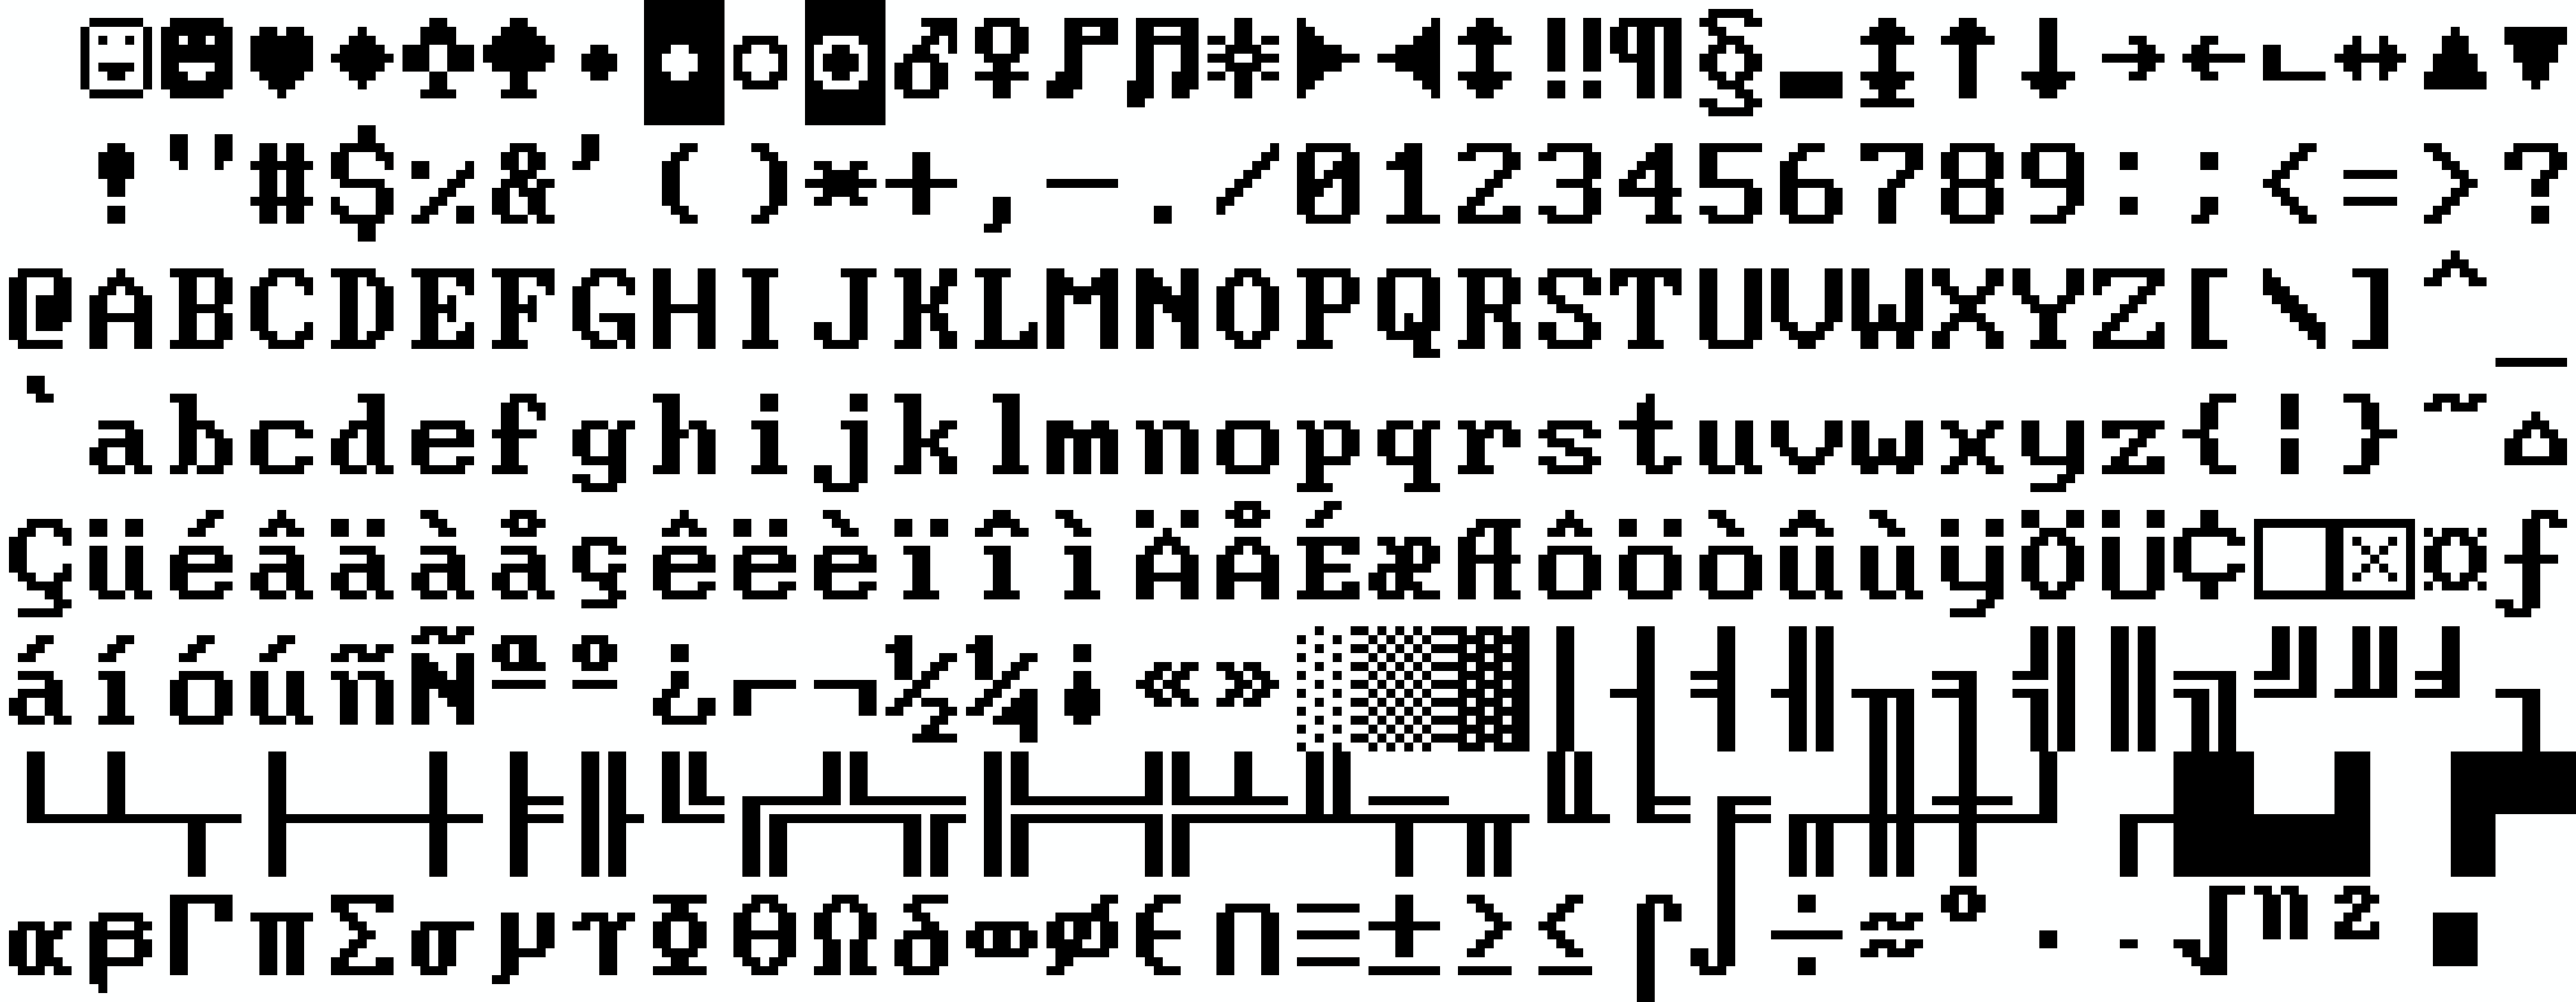
\includegraphics[width=\cpimagew]{mda.png}\end{center}

Character 0x9E (currency symbol) and 0xFA (middle dot) can be accessed with following Lua constants: \emph{MONEY} and \emph{MIDDOT}. See \emph{Lua Globals} > \emph{Constants} section.

\section{Accepted Control Sequences}

\begin{tabularx}{\textwidth}{c X c X}
	\textbf{\large No.} & \textbf{\large Description} & \textbf{\large No.} & \textbf{\large Description}
	\\ \\
	\endhead
	7 & BEL. Emits short tone. & 8 & BS. Moves cursor to left 1 character.
	\\ \\
	9 & TAB. Inserts appropriate horizontal space. Tab size is variable. & 10 & LF. Prints a new line.
	\\ \\
	12 & FF. Clears everything in screen buffer and moves cursor to (1, 1) & 13 & CR. Moves x coordinate of cursor to 1.
	\\ \\
	16 & DLE. Sets foreground colour to the default STDERR colour. & 127 & DEL. Backspace and deletes one character.
	\\ \\
	17 & DC1. Sets foreground colour to 0. (black) & 18 & DC2. Sets foreground colour to 1. (white)
	\\ \\
	19 & DC3. Sets foreground colour to 2. (dim grey) & 20 & DC4. Sets foreground colour to 3. (bright grey)
\end{tabularx}

\chapter{Lua Globals}
ROMBASIC adds global functions and constants for operability.

\section{Functions}

\begin{tabularx}{\textwidth}{l l X}
	\textbf{\large Function} & \textbf{\large Return} & \textbf{\large Description}
	\\ \\
	\endhead
	\unemph{\_G.}runScript(\textbf{fun}: str, \textbf{env}: str) & nil & Runs Lua script \textbf{fun} with the environment tag \textbf{env}.
	\\ \\
	\unemph{\_G.}bell(\textbf{pattern}: str) & nil & Strike bell (or beeper) with pattern. See section \emph{Bell Codes} for more information. Aliased to \unemph{\_G.}emitTone.
\end{tabularx}

\section{Constants}

\begin{tabularx}{\textwidth}{l l X}
	\textbf{\large Name} & \textbf{\large Type} & \textbf{\large Description}
	\\ \\
	\endhead
	\unemph{\_G.}\_TERRARUM & non-false & Indicator for multi-environment scripts.
	\\ \\
	\unemph{\_G.}EMDASH & string & EM dash represented by box-drawing character. Code 0xC4
	\\ \\
	\unemph{\_G.}UNCHECKED & string & Unchecked checkbox. Code 0x9C
	\\ \\
	\unemph{\_G.}CHECKED & string & Checked checkbox. Code 0x9D
	\\ \\
	\unemph{\_G.}MONEY & string & Currency symbol used in the world. Code 0x9E
	\\ \\
	\unemph{\_G.}MIDDOT & string & Middle dot used in typography. Code 0xFA (note: 0xF9 is a Dot Product used in Mathematics)
	\\ \\
	\unemph{\_G.}DC1 & string & Ascii control sequence DC1. Used to change foreground colour to black.
	\\ \\
	\unemph{\_G.}DC2 & string & Ascii control sequence DC2. Used to change foreground colour to white.
	\\ \\
	\unemph{\_G.}DC3 & string & Ascii control sequence DC3. Used to change foreground colour to dim grey.
	\\ \\
	\unemph{\_G.}DC4 & string & Ascii control sequence DC4. Used to change foreground colour to bright grey.
	\\ \\
	\unemph{\_G.}DLE & string & Ascii control sequence DLE. Used to change foreground colour to terminal's default error text colour.
	\\ \\
	computer.prompt & string & Default text for prompt input indicator.
	\\ \\
	computer.verbose & bool & Sets whether print debug information to the console.
	\\ \\
	computer.loadedCLayer & table & List of names of compatibility layers has been loaded.
	\\ \\
	computer.bootloader & string & Path to the boot file. Should point to the EFI (/boot/efi).
	\\ \\
	computer.OEM & string & Manufacturer of the computer. If you \emph{are} a manufacturer, you may want to fill in this variable with your own company's name.
	\\ \\
	computer.emitTone(\textbf{len}, \textbf{freq}) & nil & Generates square wave. \textbf{len} is integer, in milliseconds, \textbf{freq} is number, in Hertz.
\end{tabularx}

\section{Bell Codes}

Bell Codes are patterns for driving bell/beeper. Each code is followed by short break of 50 milliseconds.

\begin{tabularx}{\textwidth}{l X l X}
	\textbf{.} (dot) & Short emitTone. 80 ms & \textbf{-} (dash) & Medium emitTone. 200 ms
	\\ \\
	\textbf{=} (equal) & Long emitTone. 500 ms & \textbf{,} (comma) & Short break. 50 ms
	\\ \\
	(space) & Break. 200 ms
\end{tabularx}
\subsection{Changes from Generic Lua Environment}
\begin{itemize}
\item io library is limited to io.read (read a line from keyboard) and io.write (print without new line). Use \emph{Filesystem} API for file I/O jobs.
\end{itemize}

\chapter{Machine}
The Machine API provides means to control the host machine.

\begin{tabularx}{\textwidth}{l l X}
	\textbf{\large Function} & \textbf{\large Return} & \textbf{\large Description}
	\\ \\
	\endhead
	machine.milliTime() & int & Returns how many time the machine is up, in milliseconds (one thousandth of seconds).
\end{tabularx}


\part[Compatibility Layers---ComputerCraft]{{\LARGE Compatibility Layers} \\ ComputerCraft}

\chapter{Bit}
The Bit API is for manipulating numbers using bitwise binary operations. The ROMBASIC already comes with Lua's bit32 library so make sure to use that for your casual usage.

\section{Functions}

\begin{tabularx}{\textwidth}{l X}
	\textbf{\large Function} & \textbf{\large Notes}
	\\ \\
	\endhead
	bit.blshift(n, bits) & Alias of bit32.lshift(n, bits)
	\\ \\
	bit.brshift(n, bits) & Alias of bit32.arshift(n, bits)
	\\ \\
	bit.blogic\_rshift(n, bits) & Alias of bit32.brshift(n, bits)
	\\ \\
	bit.bxor(m, n) & Alias of bit32.bxor(m, n)
	\\ \\
	bit.bor(m, n) & Alias of bit32.bor(m, n)
	\\ \\
	bit.band(m, n) & Alias of bit32.band(m, n)
	\\ \\
	bit.bnot(n) & Alias of bit32.bnot(n)
\end{tabularx}

\chapter{Colors}
The Colors API allows you to manipulate sets of colors. This is useful in colors on Advanced Computers and Advanced Monitors. British spellings are also supported.

\subsection{Constants}

When the colours are used in ComputerCraft's Term API, nearest console colours will be used. Below is the table of colours coded with their substitutions.

\begin{tabularx}{\textwidth}{l l l l}
	colors.white & colors.\textcolor{orange}{orange} & colors.\textcolor{magenta}{magenta} & colors.\textcolor{cyan}{lightBlue}
	\\ \\
	colors.\textcolor{yellow}{yellow} & colors.\textcolor{lime}{lime} & colors.\textcolor{tan}{pink} & colors.\textcolor{dimgrey}{gray}
	\\ \\
	colors.\textcolor{brightgrey}{lightGray} & colors.\textcolor{cyan}{cyan} & colors.\textcolor{purple}{purple} & colors.\textcolor{blue}{blue}
	\\ \\
	colors.\textcolor{brown}{brown} & colors.\textcolor{green}{green} & colors.\textcolor{red}{red} & colors.\textcolor{black}{black}
\end{tabularx}

Note that pink is understood as \textcolor{tan}{tan} when it is used, lightBlue and cyan are merged to \textcolor{cyan}{cyan}.

\subsection{Functions}

All three functions are not supported, as there is no bundled cable thus there is no use of them.

\chapter{Term}

\chapter{Filesystem}



\part[Compatibility Layers---OpenComputers]{{\LARGE Compatibility Layers} \\ OpenComputers}



\part{Peripherals}

\chapter{Line Printer}
The line printer is a printer that operates on line basis. It only prints text in line-by-line, hence the name, on almost endlessly long roll of papers; it has no notion of page, it just prints. If you want some pages to keep, you must tear them out yourself.

Line printers do not work indefinitely; ignoring the obvious depletion of ink, belt for loading paper will be out of service on about 50 000 lines of printing, give or take a few, or paper will jam if the printer had struck with the unluckiness.

\subsection{Functions}

\begin{tabularx}{\textwidth}{l l X}
	\textbf{\large Function} & \textbf{\large Return} & \textbf{\large Description}
	\\ \\
	\endhead
	lp.print(string) & nil & Prints a line of string.
	\\ \\
	lp.scroll(\textbf{n}: int) & nil & Scrolls the paper by \textbf{n} lines.
	\\ \\
	lp.status() & int & Returns a status of the line printer.
	\\ \\
	lp.reset() & nil & Resets the line printer.
\end{tabularx}

\chapter{PSG}
%\input{peri_psg}



\part{References}

Some of the texts are taken from following sources:

\begin{itemize}
\item Lua Manual version 5.2, Lua.org, POC-Rio
\item ComputerCraft, dan200
\item OpenComputers, MightyPirates
\end{itemize}

\afterpage{\pagestyle{empty}\null\newpage}

\end{document}